%\documentclass[preprint]{aastex}  % USE THIS TO MAKE BIB, THEN FORMAT USING EMULATEAPJ
\documentclass[twocolumn,numberedappendix]{emulateapj}
\shorttitle{PSA64}
\shortauthors{Ali, et al.}

\usepackage{amsmath}
\usepackage{graphicx}
\usepackage[figuresright]{rotating}
%\usepackage{rotating}
\usepackage{natbib}
%\usepackage{pdflscape}
%\usepackage{lscape}
\citestyle{aa}

\def\b{\mathbf{b}}
\def\k{\mathbf{k}}
\def\r{\mathbf{r}}
\def\q{\mathbf{q}}
\def\b{\mathbf{b}}
\def\kp{\mathbf{k}^\prime}
\def\kpp{\mathbf{k}^{\prime\prime}}
\def\V{\mathbb{V}}
\def\At{\tilde{A}}
\def\Vt{\tilde{V}}
\def\Tt{\tilde{T}}
\def\tb{\langle T_b\rangle}
\newcommand{\vis}{\mathbf{v}}
\newcommand{\x}{\mathbf{x}}
\newcommand{\xhat}{\hat{\mathbf{x}}}
\newcommand{\A}{\mathbf{A}}
\newcommand{\N}{\mathbf{N}}
\newcommand{\rhat}{\hat{\mathbf{r}}}

\begin{document}
\title{PSA-64 Power Spectrum}

\author{
Zaki S. Ali\altaffilmark{1},
Aaron R. Parsons\altaffilmark{1,2},
Jeff Zheng,
Jonathan C. Pober\altaffilmark{4},
James E. Aguirre\altaffilmark{3},
David R. DeBoer\altaffilmark{2},
Daniel C. Jacobs\altaffilmark{8},
Adrian Liu\altaffilmark{1},
David F. Moore\altaffilmark{3}
% XXX if includes paper data, needs full author list
}

\altaffiltext{1}{Astronomy Dept., U. California, Berkeley, CA}
\altaffiltext{2}{Radio Astronomy Lab., U. California, Berkeley, CA}
\altaffiltext{3}{Dept. of Physics and Astronomy, U. Pennsylvania, Philadelphia, PA}
\altaffiltext{4}{Physics Dept.  U. Washington, Seattle, WA}
\altaffiltext{8}{School of Earth and Space Exploration, Arizona State U., Tempe, AZ}

\begin{abstract}
\end{abstract}

% XXX fringe weighting profile
% XXX delay spectrum not violated by freq-dependent fringe rate weights

\section{Introduction}
The Donald C. Backer Precision Array for Probing the Epoch of Reionization
(PAPER) is a dedicated experiment to measure the power spectrum of highly
redshifted 21 cm emission during the Epoch of Reionization. PAPER is but one
experiment that aims to detect this faint signal. Other telescopes that have the
same goal are the Giant Meter-wave Radio Telescope (GMRT), the LOw Frequency
ARray (LOFAR), and the Murchison Widefield Array (MWA). PAPER currently consists
of 128 dual-polarization antennaes in a 100-200MHz band out in the Karoo desert
in South Africa. 

The current best upper limit on 21 cm signal level is at $(41 mK)^{2}$ at
$k=.27 h \text{Mpc}^{-1}$ which was measured by PAPER in a 32 antenna redundant
configuration (\ref{parsons_et_al2014a}). This limit was acheived by using the
delay-spectrum technique to remove foregrounds and using the  maximum
redundancy array to repeatedly measure the same fourier mode, boosting
sensitivity. In this analysis we employ the same techniques mentioned, as well
is introduce an optimal fringe-fringe rate filter to  boost sensitivity and
make use of improved calibration via the Omnical redundant calibrator package. 

The paper is outlined as follows. In section \ref{sec:observations} we describe
the observations used in this analysis. In \ref{sec:improvements} we discuss the
improvements in this pipeline with respect to the previous analysis of PSA-32
\cite{parsons_et_al2014a}. We then move on to the data analysis pipeline in
section \ref{sec:analysis}. Seciton \ref{sec:results} describes the results of
 our efforts and provides new contraints on EoR. We conclude in
\ref{sec:conclusion}.


\section{Observations}\ref{sec:observations}
Here, we describe the features of the data set used in this analysis. 
The observations discussed in this paper were taken when PAPER consisted of 64
dual polarization antennas deployed in the Fall of 2012.  The antennas were
arranged in a maximally redundant configuration as seen in Figure
\ref{fig:antenna_positions}). We rely on all
of the baselines for the calibration procedure to , but only using a
subset of the baselines for the power spectrum analysis. The columns are
separated by 30 meters and the rows by 5 meters. For the power spectrum analysis
we are using the baselines that correspond to the width between two columns
(e.g.  49-41) as well as those that correspond to over and up and down one
antenna (e.g. 10-41 and 10-58, respectively). These 154 baselines are
instantaneously redundant and therefore they measure the same Fourier modes on
the sky. Within a single group of the three types of baselines above, the
measurements add coherently, whereas between groups they add in quadrature.
Having repeated measurements of the same baseline type greatly increases
sensitivity. 

The observation of this 64 antenna data set spanned a 135 day period that
commenced on 2012 November 8 (JD62456240) and ended  2013 March 23 (JD62456375). 
Each baseline instantaneously measured the 100-200 MHz band which was divided
into 1024 frequency channels of resolution 97.66 kHz and integrated for 10.7
seconds. In this analysis we analyze observations that spanned, in local
siderial time (LST), a range of 1:00 to 10:00 hours. This range corresponds to
the "EoR cold patch", in which galaxtic synchrotron power is minimal (away from
the center of the galaxy).
%XXX lst range will change.

\begin{figure*}[!t]\centering
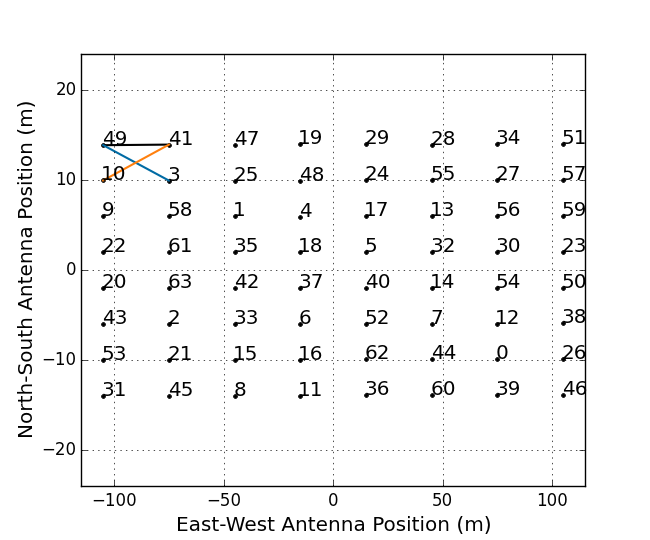
\includegraphics[width=1.85\columnwidth,height=\columnwidth]{plots/antenna_positions.png}
\caption{Antenna positions for the PAPER 64 observation run.}
\label{fig:antenna_positions}
\end{figure*}

\section{Summary of Improvements from PSA32}
In comparison to the previous PAPER pipeline (see \cite{parsons_et_al2014a}),
this analysis took a slightly different approach which included some critical
steps to improve our upper limit. In short, the improvements included using a
new, refined redundant calibration method (Zheng 2014), increasing the width of
the wideband delay filter that removes smooth spectrum foregrounds, weighting
the lst binned data sets, and optimal fringe rate filtering. In section
\ref{sec:analysis}, we dicuss each of the improvements in more detail.

Figure \ref{fig:step_through_pspec} (TBD) shows the power spectra when each of
the steps mentioned above are turned off and for the one where all of them are
turned on. We can see the gradual improvement of the power spectra (hopefully).


%A more rigorous calibrations. Forward Ref.
%omnical
%lstbinning with chi-sq weighting
%horizon cut at 200ns = 100 + 100 (instead of 100 + 15)
%optimal fringe-rate filtereing
%want the 4(5?) figures in this section. Incrementally step back through improvement points.


\section{Analysis}
Here we describe the analysis pipeline of the data set obtained in 2012/2013
observing season. 
Data was first run through a preprocessing compression pipeline which reduces
the volume of the data by a factor of forty. Afterwards we calibrate the
relative phases of our array on the basis of redundancy using a logcal approach
in delay space, and then get the absoultue phase calibration by fitting. We then
set the flux scale of our observations by using Pictor A. The logcal done above
was a rough estimate of the phase calibration and hence we used Omnical to get
the calibrations to higher accuracy. This was a major difference in the pipeline
from previous iterations on PAPER data. We then remove foregrounds using the
delay filtering technique and form power spectra. The detalis of the above are
discussed below and figure \ref{fig:analysis_pipeline} shows a block diagram of
the analysis pipeline.

\subsection{Preprocessing Compression}
As the number of elements in an interferometer increase, the amount of data to
be stored increase by order $\Omega{N^{2}}$, where $N$ is the number antennas.
Hence, a doubling of an array, increases the data volume by a factor of 4. For
large $N$ arrays, this volume of data could be prohibitive to store on disks and
can become a bottleneck in data analaysis due it being slow to comb trhough the
data. New methods of data compression and analysis that can either
reduce the data volume or provide a streaming analysis pipeline are needed for
these large arrays. 

PAPER employs a compression method that employs the use of a delay/delay-rate
filter described in \cite{parsons_backer2009}. In short, the algorithm makes use
of the fact that for a given maximum baseline (in our case, 300 meters), there is
a maximum delay sky emission can enter a baseline, given by 

\begin{equation}
    \tau_{g} < \frac{|\mathbf{b}|}{c}.
\end{equation}

Hence, if we filter out delays that are higher than this maximum delay, we can
down sample the frequency axis by the Nyquist rate. This is where reduction in
data volume comes in.  Similarily, in delay-rate space, there is a maximum
delay rate a model point source can have, which is given by, 

\begin{equation}
    -\omega_{\oplus}\frac{|b_{y}|}{c} \leq \frac{d\tau_{g}}{dt} 
                                     \leq \omega_{\oplus}\frac{|b_{y}|}{c}.
\end{equation}

This equation is valid at an Hour Angle of $h = 0^{\circ}$ and and a declination
of $\delta = 0^{\circ}$, where the maximum delay-rates occur. 
By filtering out delay-rates that are outside of this range, we are removing
sources that have a high rate of change with respect to the rotation of the
earth. That is fast transient sources will be removed. We can then decimate in
time with respect to the Nyquist rate, giving us another dimension to decrease
data volume. For greater detail, see \cite{parsons_et_al2014a}.

Note that the only parameter the compression described above depends on is a baseline
orientation and length. For this dataset, we used a baseline oriented along the
east-west direction at a latitude of $-30^{\circ}$ with a length of
300 meters.
Applying the compression to a 10 minute file consisting of 1024 channels over a
100 MHz bandwidth and 60 time samples consisting of 
10 second integrations, outputs a file consisting of 203 channels over the same
bandwidth and 14 time samples consisting of 42.8 second integrations. This is a
factor of 20 reduction in data volume. Originally, this dataset required 40 TB
of storage in its raw form. After compression, this data set required 2TB of
storage. This reduction in data volume greatly facilitated analysis (how?) and
allowed us to use shredder (describe shredder).

(Show plot of raw data and compressed data? )


\subsection{Calibrations}
\subsubsection{Overview}
As the name suggests, redundant calibration (\cite{liu_et_al2010},
\cite{zheng_et_al2014}) uses redundancy within the array to solve for relative
phases and gains of the antennas. To explain redundant calibration, suppose that
the baseline between antennas $i,j$ measure a visibility $v_{ij}$, then we have 

\begin{equation}\label{eqn:redcal}
    v_{ij} = g_{i}g_{j}^{*}y_{i-j} + n_{ij},   
\end{equation}
where $g_{i}$,$g_{j}$ are the complex gains due to antenna $i$ and antenna $j$,
respectively, $y_{i-j}$ is the true visibility measured by perfect antennas
$i$,$j$ for the given baseline type, and $n_{ij}$ is the residual noise from
the baseline.  If the number of baselines of a given type is much greater than
the number of baselines types this problem is over constrained and $g_{i}i$,
$g_{j}$, and $y_{i-j}$ can be solved for. PAPER is in this limit due to the
maximally redundant configuration as shown in figure \ref{fig:antenna_pos}. 

Redundant calibration comes in two flavors: log calibration and linear
calibration. Log calibration, or logcal for short, takes the logarithm of
equation \ref{eqn:redcal} to give a linearized system. Hence, solutions can be
solved for by using standard linear algebra techniques. However, this method is
biased. On the other hand linear calibration, or lincal for short, is an
unbiased method of solving for the complex gain solutions. In this method
equation \ref{eqn:redcal} is Taylor expanded about an initial guess for the
$g_{i}$'s and $y_{i-j}$'s to give a linearized equation which can be used to
solve for the complex gains and sky model. 

In this analysis we used a logcal algorithm based in delay space to get a rough
calibration of the dataset. This was followed by an absolute calibration to set
the overall phase and flux scale using a self calibration. We used model phase
centers of Pictor, Fornax A, and Crab Nebula. The absolute amplitude is set
by the flux of Pictor A found in \cite{jacobs_et_al2013}, whose spectrum is
defined by 
\begin{equation}
    S_{\nu} = 382(\frac{\nu}{150 MHz})^{-.76} Jy.
\end{equation}

Finally, we used the Omnical calibration package to do another round of
redundant calibration to get even more accurate calibration parameters.

\subsection{logcal-for lack of a better title}
We first perform the same calibration that was
done in \citep{parsons_et_al2014a}. That is, we use redundancy to do a relative
phase\footnote{In actuality, we solve for delays to get around phase wrapping
issues. These delays are applied to visibilities as $e^{2\pi{i}\tau\nu}$}
calibration between antennas, which removes the electrical delays from cables in
the signal path. Due to redundancy, we can calibrate out all of the per-antennas
delays in the signal path relative to two delay parameters which we call
$\tau_{ns}$ and $\tau_{es}$. These delays are the relative electrical delays
that correspond to baseline delays in the north-south and east-west component
for 2 reference baselines (49-10 and 49-41,respectively). These solutions were
then applied to the data set which was calibrated again with Omnical. 

The application of this calibration to the data set before Omnical was needed
because in order to calibrate accurately, Omnical needs to have a rough estimate
for the calibration solutions for every antenna. In \cite{zheng_et_al2014}, a
model of the sky was used in order get the rough estimate of the solutions.
Here, we use actual sky data to get the rough calibration. Because the solutions
are derived from the instrument, we can incorporate into the solutions antenna
based variations. 
 
The antenna based
delay solutions vary as much as a couple nanoseconds day to day when solutions
are averaged over hour long timescales withing a day. However, the variations in
solutions is worse when only averaging over ten minute time scales. Therefore
need for better calibration is requred.  We use self calibration to derive the
two unknow parameters, $\tau_{ns}$ and $\tau_{ew}$, by using the Crab Nebula,
Fornax A, and Pictor A.

Note that there is no possibility of signal loss (see \citep{parsons_et_al2014a}).

\subsection{Gain Calibration}
Gain calibration was derived on the basis of redundancy and self calibration.
The phase calibrations described above, simultaneously also calibrated for the
relative gain variation between antennas. Again we can only calibrate to a fiducial
antenna (49) whose gain is defined as unity. We then perform a self calibration
to set the flux scale to Pictor A whose spectrum is derived in
\citep{jacobs_et_al2013}. We use the same methods describes in \citep{parsons_et_al2014a}.

Figure \ref{fig:bmfom_pic} shows that dataset beamformed to Pictor A, with log
janskies on the y axis and lst on the xaxis for a frequncy of .1 + (120/203)*.1/203. 
As can be seen, the day to day variation in the formed beam has a fractional
spread of about 10$\%$.  This shows the stability of the instrument and the well
behaved calibration solutions derived above. 

\subsection{Omnical}
(How did we know that our calibrations were not good enough? Because of the power
spectrum? PSA32? We did beamform data to pictorA and say that vs LST, the
beamform matched well day to day with a fractional spread of about 10$\%$) 

The complex gain solutions found in the previous calibration pipeline were
averaged together in time and one solution per frequency was used for the array.
This jived with the philosophy that the array was stable in time and frequency.
However, upon further review of this data set, it seemed more and more likely
that this was not the case anymore. (Is this even true? What specifically? Think
Man!) 

Due to clues that showed that our data set had time dependent calibration
solutions, it was imperative that we do a better job at calibrating our array.

The Omnical redundant calibrator
package\footnote{https://github.com/jeffzhen/omnical} (omnical) performs
redundant calibration for every time and frequency in a dataset using both
logcal and lincal methods as described in \cite{zheng_et_al2014}. It also
contains methods on the quality of the solutions by providin a chi-square for
the fits to the data. 

For this dataset, omnical first performed a logcal (again) to attain a solution
per time and frequency. This solution was passed to lincal which iteratively
solved for the complex gain solutions. The convergence criteria was when the
$\chi^{2}$ decreased by less than $.01\%$. The $\chi^{2}$ for the fit used in
Omnical is given by 
\begin{equation}
    \chi^{2} = \sum_{ij}|v_{ij} - y_{i-j}g_{i}^{*}g_{j}|^{2},
\end{equation}

which differs from normal nomenclature because we are not inverse varaince
weighting. Note that this $\chi^{2}$ is summing over all baselines and hence 
giving more weight to higher gains. Note that omnical fits for each of the
complex gains and the model visibility, $y_{i-j}$,  for a unique baseline.
Using this information, figure \ref{fig:chi_2} shows that the $\chi^{2}$ is close
to 1 for all channels and time (for this day of data). need noise model for
this.

Figure \ref{fig:gain_solutions} shows the gain solutions output by omnical. The
amplitude of the gains are roughly order unity through out. These are relative
gains between antennas and hence the over flux scale set to Pictor A is still
valid. The absolute calibration is still valid. 

Since Omnical outputs a model visibility of what a unique baseline should
measure, which is derived from the data by removing all of the variation between
unique types of baselines and averaging, we are able to use these outputs as our
dataset. Infact, this is what is done. 
%waterfalls of chi squared and solutions.
%day to day repeatability.
%The output of the omnical - 
%




\subsection{WB delay filtering}
After calibration, we form our estimate of stokes I by combining the two linear
polarizations as $V_{I} = .5 (V_{xx} + V_{yy})$, where $V{xx}$ and $V{yy}$ are
the visibilities for the $xx$ and $yy$ linear polarizations for the same
antenna. We then perform 


Galactic synchrotron and extragalactic point sources, generally foregrounds,
greatly contaminate the EOR signal. They are 5 orders of magnitude (in K)
(Pober 2013a) above the expected level of EOR and can hide low order RFI events
and cross-talk. Removing foregrounds is a critical step in getting to a
detection of EoR. In addition to dominating the EOR signal, foregrounds can
corrupt higher-order $k$ modes in the power spectrum measurement from the
sidelobes arising from RFI flagging and the finite bandwidth used in the line
of sight Fourier transform (corresponding to $k_{\parallel}$). 

PAPER uses the delay filtering technique described in \citep{parsons_et_al2012b} to
remove smooth spectrum foregrounds that mask EoR. Taking the fourier transform
along the freuqncy axis for a visibility, which defines the delay transform,
maps sky emission in to delay space. Flat spectrum sources in this space are
show up as dirac delta functions. This method of localizing sources relies on
the fact that for a given baseline, there is a maximum delay points on the sky
can come in at. This maximum delay is given light travel time between the two
antennas in a baseline. Physically, this corresponds to emission from the
horizon. Therfore, all sky emission is localized to this "horizon limit."

Following the technique described in \citep{parsons_et_al2012b}, the delay transform
of a visibility takes the form 

\begin{align}\label{eqn:delay_transform}
    \tilde{V} &= \int{W(\nu)S(\nu)V(\nu)e^{-2\pi{i}\tau\nu}d\nu} \\
              &= \tilde{W}(\tau) \ast \tilde{S}(\tau) \ast \tilde{V}(\tau) \ast
                 \delta(\tau_{s} - \tau)
\end{align}
where $V(\nu)$ is the visibility measured, $W(\nu)$ is a blackman-harris
windowing function and $S(\nu)$ is the weighting function that encodes the
boolean flags for the data. As mentioned above, a flat spectrum source will show
up as a delta function in delay space, but if there is any spectral structure,
the shape of that structure will become a convolving kernel in delay space,
increasing the footprint of the source in delay space. Since foregrounds are
modeled as having a smooth spectrum, the convolving kernel is narrow in delay
space, whereas EoR is expected to have a large amount of frequency structure
and hence has a wide convolution kernel, scattering signal outside of the
horizon limit. By removing smooth spectrum foregrounds by fourier filtering in
delay space, we can remove bright foregrounds that keep us from detecting EoR.

On a practical note, the boolean flags in equation \ref{eqn:delay_transform} are
usually not regularily sampled and create structure in delay space due to the
uneven sampling and sharp frequency structure. This will cause the normally
localized smooth spectrum foregrounds to scatter emission in to otherwise
uncorrupted delay modes. As described in \cite{parsons_backer2009}, we use a
CLEAN algorithim that treats the boolean flags as a sampling function and
iteratively fits the brightest peak in delay space to some threshold. This does
an excellent job in filling in the gaps of the delay transform, due to the
exactly known sampling function, and returns a model of the data without any
flags. 

In the above CLEAN, we restrict the clean components to fall within 15 ns beyond
the horizon. This limit lets CLEAN model foreground emission pushed beyond the
horizon (due to spectral structure). This CLEAN model is then subtracted from
the delay transform and suppresses smooth spectrum foreground. As seen in figure
\ref{fig:wideband_delay_removal}, this filter is responsible for 3 orders of
magnitude of foreground removal (in mK) within the horizon. For our 30 meter baselines
used in this analyisis, the horizon limit is at 100 nanoseconds in delay domain,
which at a frequency of 164 MHz, corresponds to $k = \pm .057 h MPc^{-1}$.
Talk about signal loss.
Using the entire bandwidth increases the degree of foreground separation and is
impereative to get the best estimate of foreground isolation. We apply the delay
transform defined above to every baseline over the entire 100 Mhz. Figure
\ref{fig:delaytransform} shows the localization of foregrounds for a 30 meter
baseline within the horizon of 100 ns. After the filter is applied we see 3
orders of magintude in reduction of foreground isolation.  This is a factor of 6
in powerspectra! 

After the wideband delay filter, we conduct another round of RFI and crosstalk
removal which was overshadowed by the foreground signal. For RFI excision we
apply a median filter which flags above $3\sigma$. Foregrounds kept us using the
traditional method of removing cross talk which consisted of subtracting hour
long averages from each visibility. This was due to the fact that some days in
the observation had gaps in time owning to some technical difficulties during
observations. However, with foregrounds removed we were able to remove 10 minute
averages from every visibility within a file (files have a cadence of ten
minutes). Normally, hour long averages are needed for foreground contained data
to wash out the fringes from the said foregrounds to detect the static phase
bias that is crosstalk. For foreground removed data, we do not have this
complication since bright foregrounds are not dominating the average and are
able to remove the offset by subtracting shorter sums.

\subsection{Binning}

Once smooth sources have been removed and a final pass of RFI excision and
crosstalk removal have been performed, the data is averaged in local sidereal
time (LST) with bins of width 43 seconds to match the integration time of the
data. The data set consisted of 135 unevenly sampled days with the effective
number of total days being 123.57. This uneven sampling in the data set was due
to technical difficulties in the recording of disks. Future publications of this
data set will have an evenly sampled data set.

Sporadic RFI events can skew individual LST bins away from the median value of
the sky at a given LST. Therefore, we compute the median in a given LST bin for
each frequency and flag off data that is 3 sigma outside of that median before
averaging. This filter mitigates the adverse effects of RFI from dominating a
LST bin. 

\subsubsection{A noise study}
During the LST averaging, we compute the median and the variance for every LST
and frequency bin. The variance in particular is of importance becuase it allows
us to estimate the system temperature, $T_{sys}$, as a function of LST and
frequency. The variance is computed, per frequency, for all the visibilities
that are included in a given LST bin, which gives us an estimate ${I_{rms}}$,
the specific intensity in Jy, which is then converted to a $T_{rms}$ in the
usual way, 
\begin{equation}
    T_{rms} = \frac{I_{rms}\lambda^{2}}{2k\Omega}.
\end{equation}

where $\lambda$ is the observing wavelength, $\Omega$ is the size of the beam in
steradian, and $k$ is the boltzmann constant. We convert $T_{rms}$ to a system
temperature by scaling up the rms with the effective integration time and
bandwidth used. That is, 
\begin{equation}
    T_{sys} = T_{rms} \times \sqrt{\Delta{B}t_{int}}.
\end{equation}

Figure \ref{fig:tsys_lst_fq} shows the system temperature as a function of
LST and frequncy. In our "cold" patch, we find that $T_{sys}$ is around $500K$.


\begin{figure}
\centering
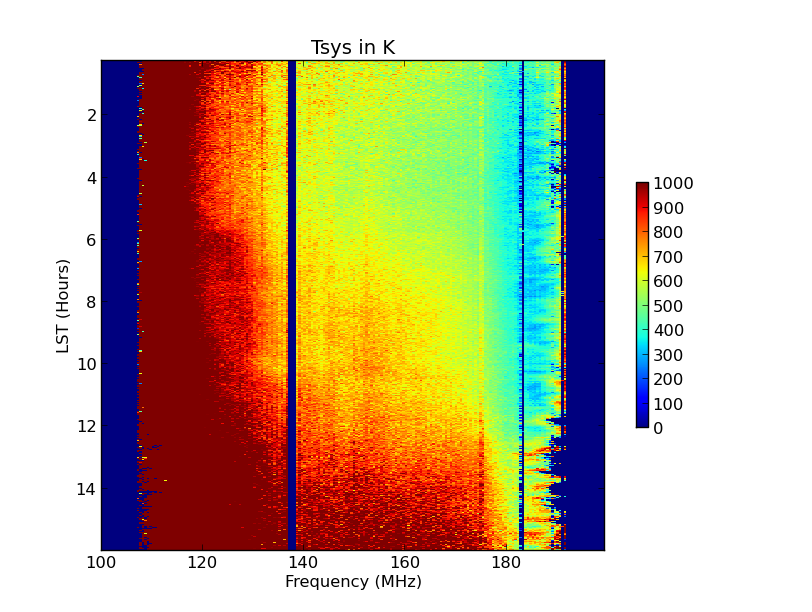
\includegraphics[width=\columnwidth]{plots/tsys_lst_freq.png}
\caption{Tsys as a function of lst and frequency. The cold spot resides in the
lst range of 1-7hours.}
\ref{fig:tsys_lst_fq}
\end{figure}






\subsection{optimal Fringe-rate filter}
Before forming power spectra we need to time average visibilities that measure
the same $k$ mode on the sky. This is the best way to combine data because we
get a $\sqrt{N}$, where N is the number of samples, gain in sensitivity. This is
in oppostion to weighting after forming power spectra, where noise beats down as
the $\sqrt{N}$. Rather than a straight averaging in time, we can do better by
using a weighted averge. Specifically, we want to upweight samples that have
higher signal-to-noise. 

This is acheived by applying a carefully crafted filter in fringe rate domain,
the fourier dual to time. Different patches on the sky correspond to different
fringe rates, for a given baseline and frequency. Maximum fringe rates are found
along the equatorial plane where zero fringe rates are found around the poles
(sources at the poles do not move through the fringes of a baselines). Sources
on the other side of the pole, corresponds to negative fringe rates, because
they move through the fringe pattern in the opposite direction. By weighing the
fringe rates sampled by a baseline by the beam response of the baseline, gives
us the optimal fringe rate filer to use for time averaging. See Parsons/Liu 2014
for a detailed discussion.

We implement the optimal fringe rate filter by first calculating the fringe rate
of everypoint on the sky and weighting it the beam of a given baseline, summing
along constant fringe rate contours. Note that because the data already has one
factor of the power beam in it, we only need to weight the fringe rates by the
power beam and not square it. That is we are upweighting fringe rate bins that
have greater signal-to-noise.  We then fit a gaussian to the optimal filter to
have a smooth function, along with tanh function for to have a smooth cut off
at the maximum fringe rate for the given baseline and frequency.  Note that
this only calculated for a given frequency and scaled to other frequencies, due
to the fact that fringe rate scales linearly with frequency via

\begin{equation}
    f_{max} = \frac{|\mathbf{b}_{eq}|}{c}\omega_{\oplus}\nu
\end{equation}


We then fourier transform the omptimal fringe rate filter and multipy by a
blackman-harris window function. This convolution kernel is then applied to 
visibilities for every baseline at every frequncy. We implement the fringe rate
filter over the span of 17163 seconds even though the full with half max of the
filter spans ~15 minutes for a 30 meter baseline. This 

Since the PAPER beam is ~45 degrees, and the array is located at a declination
of $-30^{\circ}$ the fringe rates associated with the low signal to noise (down
in the beam) correspond to very high and very low/negative fringe rates. Figure
\ref{fig:fringe_rate_cut} shows a cut of the optimal fringe rate at MHz for a 30
m east west baseline. Therfore, the implemented fringe rate filter removes some
sky signal, signal associated with fringe rates outside of the ranges shown in
Figure \ref{fig:fringe_rate_cut}. Figure \ref{fig:fr_preserved_signal} shows
that the applied filter removes sky associated with negative fringe rates and
very high fringe rates. 

\begin{figure}
\centering
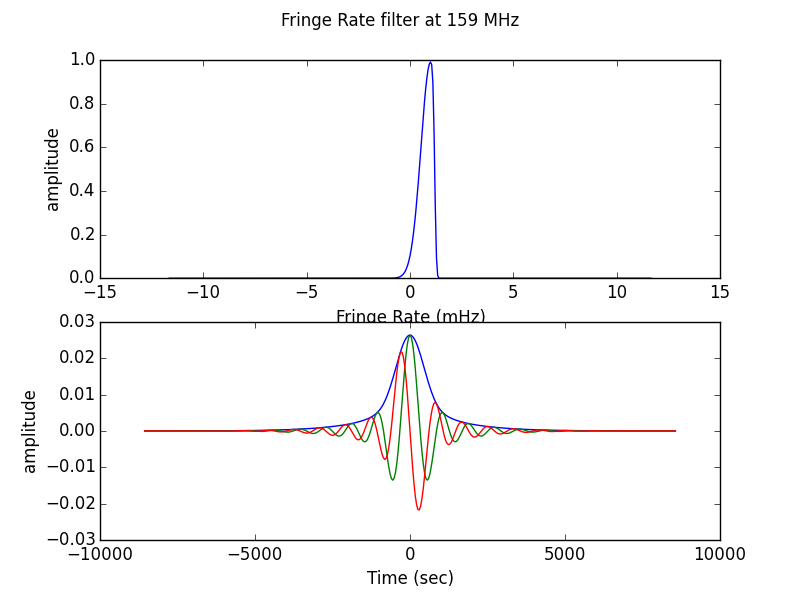
\includegraphics[width=\columnwidth]{plots/fr_filter_slice.png}
\caption{slice of a fringe rate filter at a frequency of 159MHz. Top is the
filter in fringe rate domain. The bottom consists of the corresponding time
domain filter gotten by fourier transforming and windowing with a
blackman-harris window to damp the tails.}
\label{fig:fringe_rate_cut}
\end{figure}

\begin{figure*}[t!]\centering
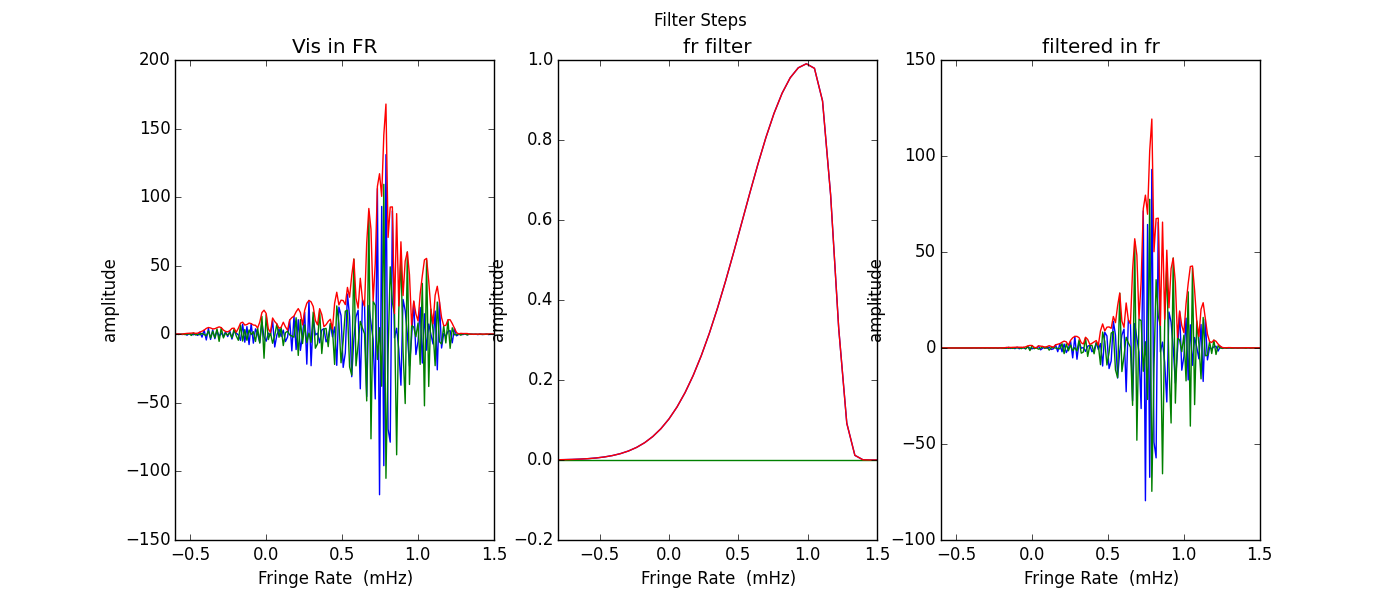
\includegraphics[width=2\columnwidth]{plots/fr_preserved_signal.png}
\caption{slice of a fringe rate filter at a frequency of 159MHz. Shown here is
the fringe-rate transform of foreground contained data for a 30 m east-west
baseline. Blue and green are the real and imaginary part, respectively and red
is the absolute valeu. Note the maximum and minimum fringerates correspond to
the theoretical minimum and maximum for a baseline of this length at 159 MHz.
The center panel shows the real (red)  and imaginary (green) parts of the fringe
rate filter to be applied. Finally, the last panel on the right shows that the
fringe rate filtered visibilities. The fringe rate filter is just a weighting
applied in fringe rate space and retains foregrounds.}
\label{fig:fr_preserved_signal}
\end{figure*}

\begin{figure}[h!]\centering
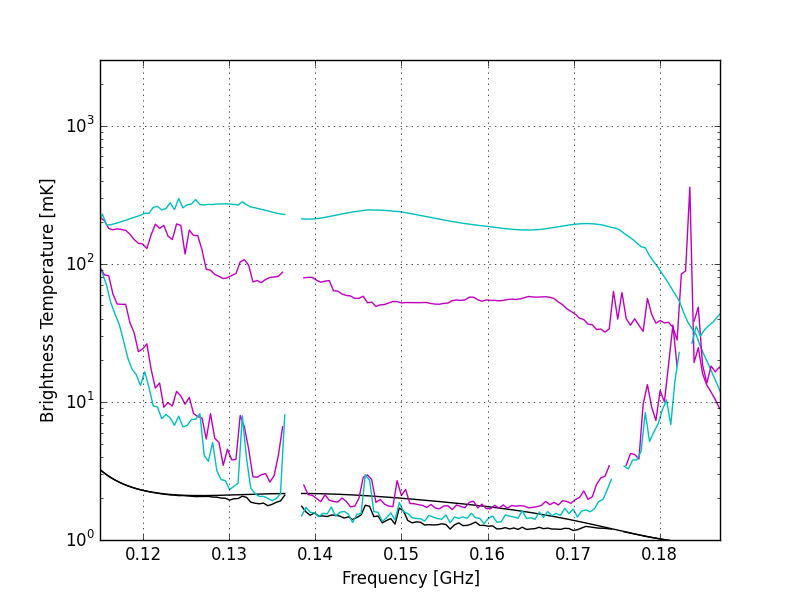
\includegraphics[width=\columnwidth, height=.8\columnwidth]{plots/noise_t_35.png}
\caption{Estimates of noise temperature. Magenta is frequncy differenced
estimate where the cyan is the time differenced estimate. All curves are
averaged over all 30m east-west baselines (56) and averaged incoherently in 43s
bins of LST from LST 3 to 5 hours with a channel bandwidth of 490 kHz.}
\label{fig:noise_t}
\end{figure}


\begin{figure}[h!]\centering
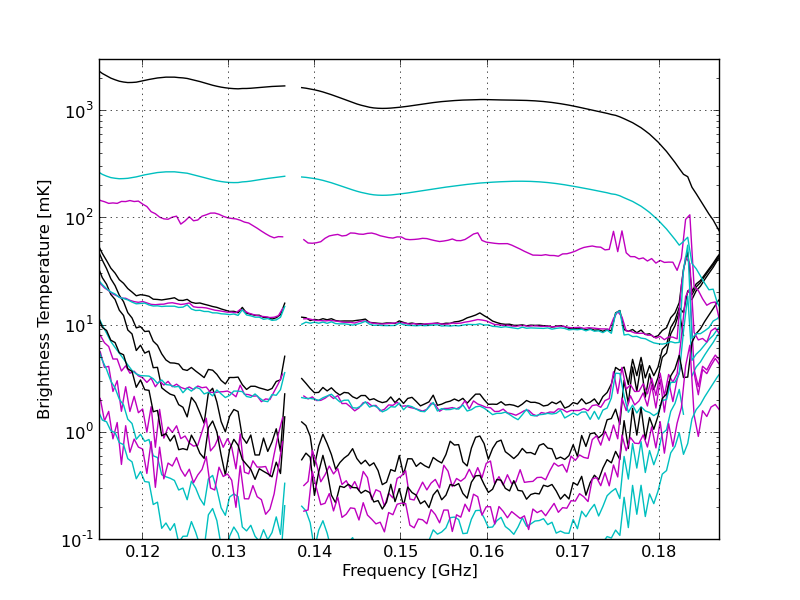
\includegraphics[width=\columnwidth, height=.8\columnwidth]{plots/noise_vs_fq_plot.png}
\caption{Estimates of noise temperature. Magenta is frequncy differenced
estimate where the cyan is the time differenced estimate. Averaged in LST from 3
to 5 hours. on uv files calibrated with omnical. fg,delay filtered, baseline
averaged, normal fringe rate filter, optimal fringe rate filtering.}
\label{fig:noise_omni_uv}
\end{figure}


\subsection{Optimal Quadratic Estimator}

\begin{figure}[h!]\centering
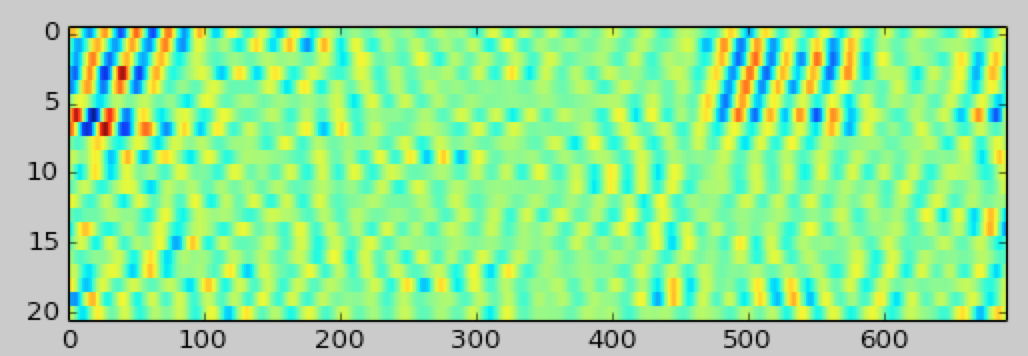
\includegraphics[width=2\columnwidth, height=.8\columnwidth]{plots/x_example.png}
\caption{Input fringe rate filtered frequncy domain data for a single baseline.}
\label{fig:x_example}
\end{figure}

\begin{figure}[h!]\centering
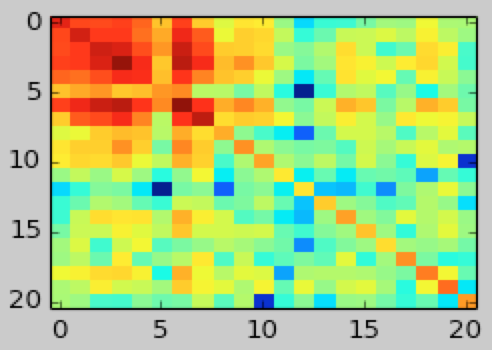
\includegraphics[width=\columnwidth, height=.8\columnwidth]{plots/C_example.png}
\caption{The covariance matix for a single baseline of the frequncy data in
figure \ref{fig:x_example}.} 
\label{fig:C_example}
\end{figure}

\begin{figure}[h!]\centering
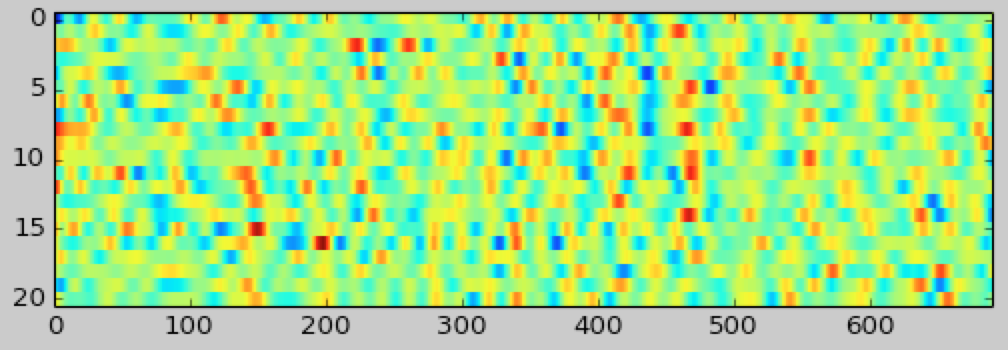
\includegraphics[width=\columnwidth, height=.8\columnwidth]{plots/_Cx_example.png}
\caption{Frequency vs. time data of a single baseline weighted by the inverse of
the covariance matrix shown in figure \ref{fig:C_example}} 
\label{fig:_Cx_example}
\end{figure}

\begin{figure}[h!]\centering
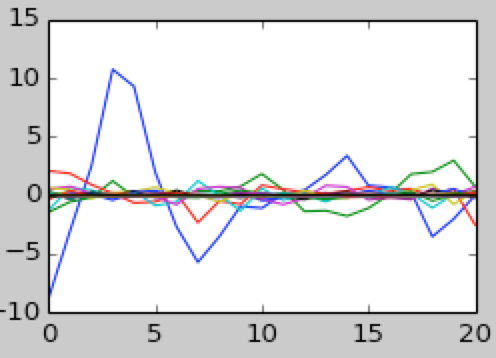
\includegraphics[width=\columnwidth, height=.8\columnwidth]{plots/lamV_example.png}
\caption{The eigeinmodes of the covariance matrix in figure \ref{fig:C_example}
weighted by their corresponding eigeinvalue.} 
\label{fig:lamV_example}
\end{figure}

\begin{figure}[h!]\centering
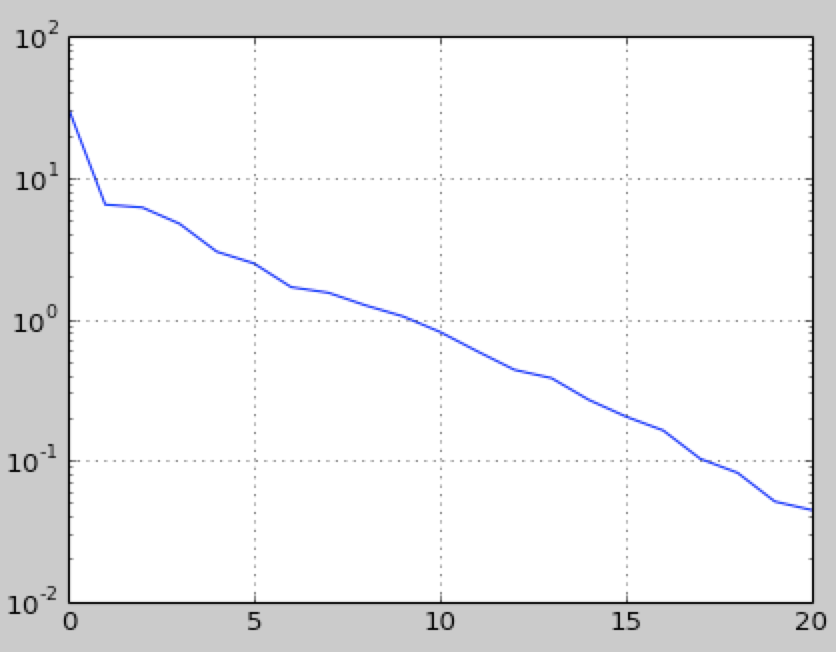
\includegraphics[width=\columnwidth, height=.8\columnwidth]{plots/lam_example.png}
\caption{The eigen spectrum of the covaraince matrix for a singel baseline.}
\label{fig:lam_example}
\end{figure}


%plots:
% filters used. 
% apply filters to foreground data. Compute fr of pica and show that we are not 
%   killing the sky.
% 


\section{Results}

\section{Science}

\section{Conclusions}


%\clearpage
%\nocite{*}
\bibliographystyle{apj}
\bibliography{biblio}

\end{document}

